\begin{figure}[H]
\centering
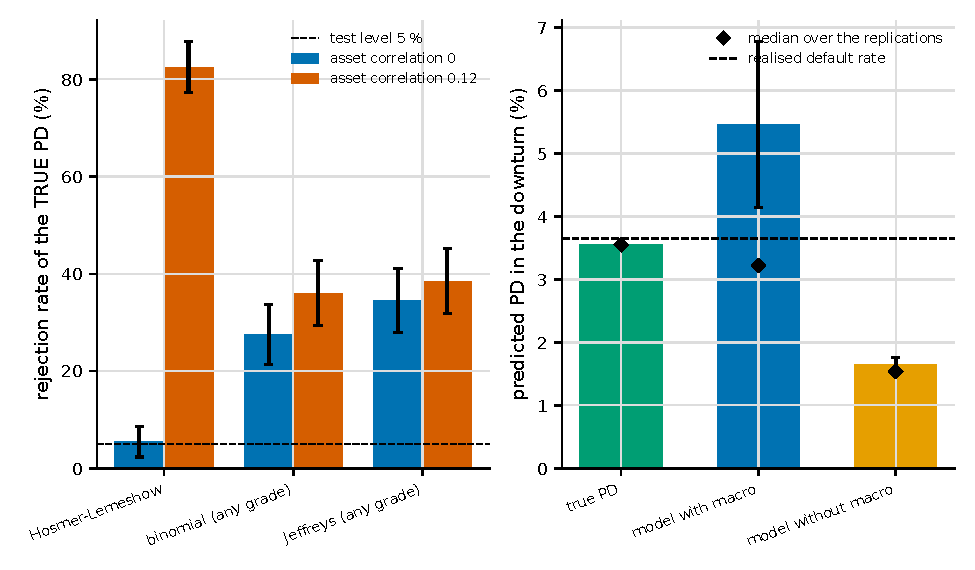
\includegraphics[width=\linewidth]{figures/fig20_calibration_drift.pdf}
\caption{Left: rejection rates of calibration tests applied to the TRUE PD of one period (20000 borrowers, M = 200), with independent defaults and with asset correlation 0.12; the per-grade tests reject if any grade does (multiple testing). Right: a downturn period (macro variable at -2 sd): mean (bars) and median (diamonds) predicted PD of the true model and of two fitted models (8 training periods) against the realised default rate; the mean of the model with the macro variable lies above its median (a noisy coefficient enters through the exponential). Hosmer--Lemeshow uses $g = 10$ degrees of freedom (the true PD is not fitted on the sample). Error bars $\pm 1.96$ se.}
\label{fig:fig20_calibration_drift}
\end{figure}
